\section{Experimental Evaluation}
\label{evaluation}

\noindent
To evaluate our model, experiments are performed on a cluster of 13 nodes, where one node serves as the master node, and the other 12 nodes serve as worker nodes. The master node has 4 CPU cores, and 6 GB of memory. Among the 12 worker nodes, 6 nodes have the same configuration: 8 CPU cores and 8 GB of memory, and the other 6 nodes have the same configuration: 12 CPU cores and 16 GB of memory. For evaluation, we ran Apache Spark using its standalone cluster mode on top of Hadoop Distributed File System (HDFS) with default 64 MB block setting. 
\noindent
For data collection, we leveraged spark event logs that are generated by the Apache Spark platform to record execution profiles and performance metrics that are directly obtained from the Spark event listeners in the Apache Spark program, and are saved in JSON~\cite{json} format. By analyzing this log file, $StageTime$ in equation (\ref{jobtime}) and $TaskTime$ in equation (\ref{stagetime}) can be easily calculated. Job $Startup$ time and job $Cleanup$ time, and stage $Startup$ time and stage $Cleanup$ time is calculated from log data as well. From task level log, task time is calculated using equation (\ref{tasktime}). Moreover, since I/O cost details are provided for each task, $TaskIOWrite$ and $TaskIORead$ is calculated using the shuffle write and read metrics to construct the I/O profile. The initial RDD is created in one of the first few stages, and each RDD block is stored in memory while the corresponding memory usage is recorded in the tasks sections of logs. Based on this information, memory consumption profile is calculated using equation (\ref{jobmem}). 
\noindent
Example applications we use to verify performance of our prediction mechanism include one non-iterative text processing algorithm: WordCount; two iterative machine learning algorithms: Logistic Regression and K-Means clustering; and one graph algorithm: PageRank. As input data, the WordCount application uses 75 GB Wikipedia dump. Logistic Regression and K-Means application use 50 GB of numerical Color-Magnitude Diagram data of galaxy from Sloan Digital Sky Survey (SDSS)\cite{sdss}. For PageRank, we use the LiveJournal network dataset from SNAP\cite{snap}, which is processed through mapping each node id into longer string to form 25 GB of data as the input for this algorithm.
\noindent
To measure the effect of simulation setup on prediction accuracy, we used two simulation setup as follows. 
In the first simulation setup, we used the whole cluster to simulate the execution. In this case, the number of CPU core $P$ is 120 and we have two cases to consider. In the first case, the sample data size is set at 7.5 GB for $P$ cores (based on 64 MB of block size) to simulate one task per core during the simulation. In this case, we assume that each task within a stage requires similar execution time. In the second case, the sample data size is set at 15 GB for $P$ cores ($2\times P$ based on 64 MB of block size) to simulate two tasks per core during the simulation. Simulating two tasks per core allows us to calculate the ratio based on the discrepancy in execution time for the first task compared to the subsequent tasks within a single stage (\ref{ratio}). 
\noindent
In the second simulation setup, we used two worker nodes of different computing capability from 12 worker nodes and kept the master node to construct a cluster of 3 nodes (as shown in Figure~\ref{fig:cluster}). In this case, the number of CPU core $p$ is 20 and we again have two cases to consider. In the first case, the sample data size is set at 1.25 GB for $p$ cores (based on 64 MB of block size) to simulate one task per core during the simulation. In this case, we assume that each task within a stage requires similar execution time. In the second case, the sample data size is set at 2.5 GB for $p$ cores ($2\times p$ based on 64 MB of block size) to simulate two tasks per core during the simulation. Simulating two tasks per core allows us to calculate the ratio based on the discrepancy in execution time for the first task compared to the subsequent tasks within a single stage (equation \ref{ratio}). 

\noindent
To evaluate the accuracy of our prediction model, we calculate the prediction accuracy for each stage and sum them as the total accuracy $R$ as follows:
\begin{IEEEeqnarray}{lCl}
\label{predict}
R = |1 - \sum_{i=1}^{M} \frac{|PredictCost_i - Cost_i|}{\sum_{j=1}^{M} Cost_{j}}|
\end{IEEEeqnarray}
Here $M$ is the number of stages for a particular job, $PredictCost_i$ is the predicted performance cost for stage $i$, and $Cost_i$ is the actual cost. Equation (\ref{predict}) can be used to calculate the prediction accuracy, and $M$ is set to 1 when computing memory cost prediction accuracy.
Our experimental result is presented below.


\subsection{WordCount}
\noindent
In the WordCount example, input data size is 75 GB. For WordCount application, there are two stages and no memory cost for the initial RDD creation. There is only I/O write cost in the first stage, and I/O read cost for the second stage. Figure~\ref{wc_accuracy} shows the accuracy for time and I/O cost prediction for different simulation setup. As can be seen in the figure, full cluster simulation achieves greater prediction accuracy. Also, as can be seen in Figure~\ref{wc_accuracy} and Figure~\ref{wc_time}, simulating two tasks per core and considering the discrepancy in execution time for the first task compared to the subsequent tasks within a single stage (equation \ref{ratio}) improves the prediction accuracy significantly. 
\noindent
For I/O cost prediction, the full scale simulation achieves much better prediction accuracy compared to the limited-scale simulation ({Figure~\ref{wc_io_w} and Figure~\ref{wc_io_r}). This may be due to the fact that the limited-scale simulation does not capture the frequent network I/O that may happen in a large-scale setup.
\begin{figure}[!t]
\centering
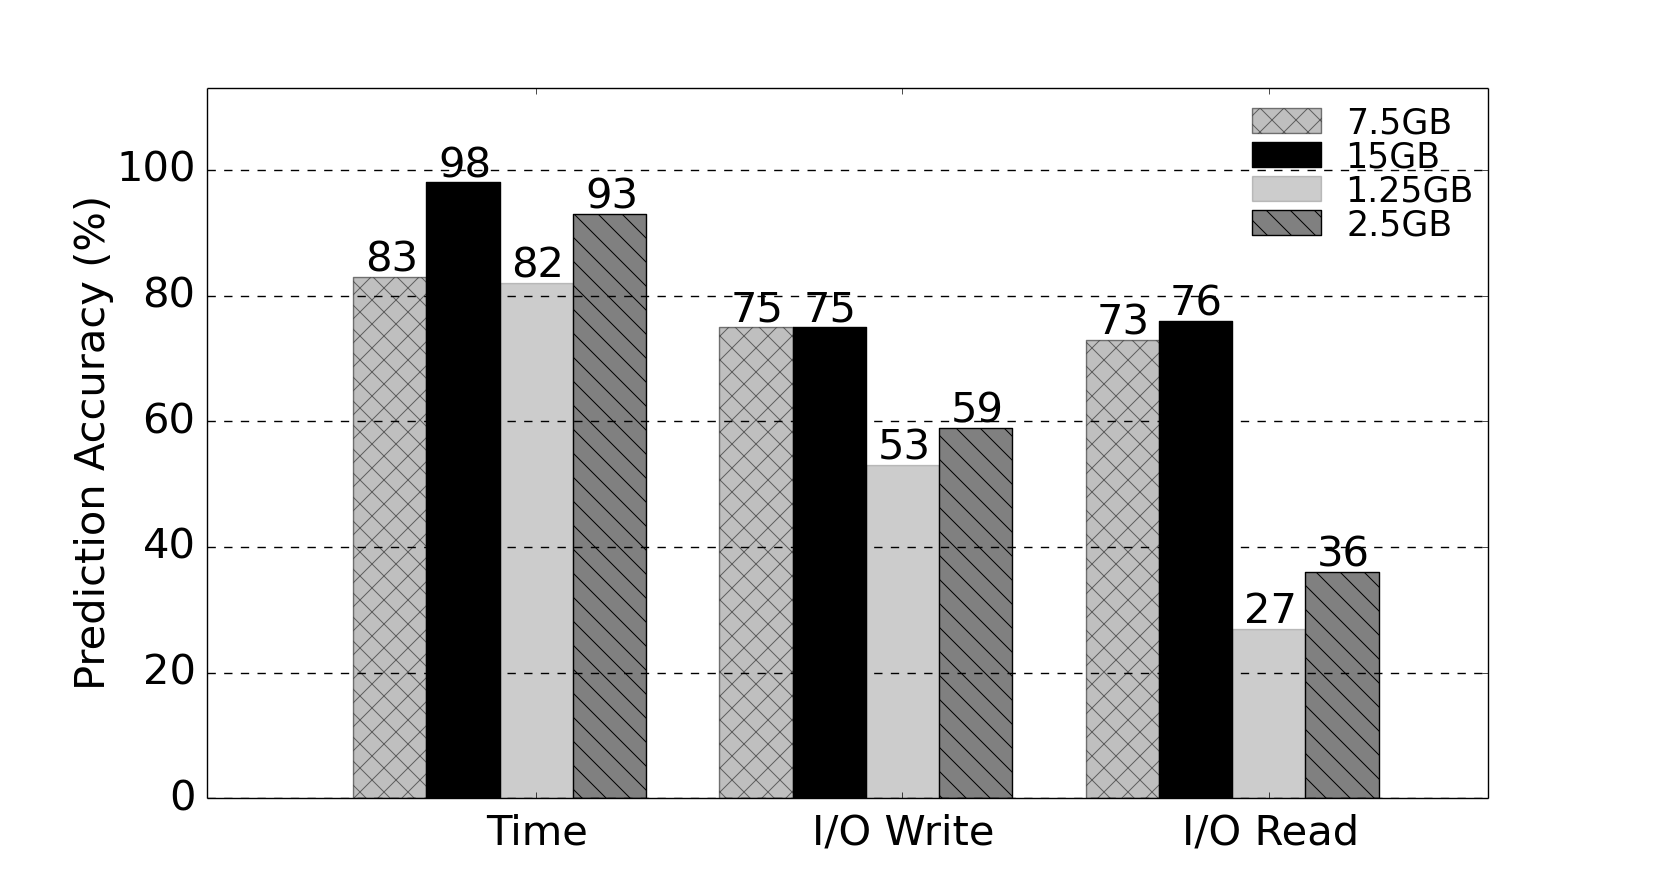
\includegraphics[width=3.5in]{figures/wc_accuracy.png}
\caption{Prediction Accuracy for WordCount}
\label{wc_accuracy}
\end{figure}
\begin{figure}[!t]
\centering
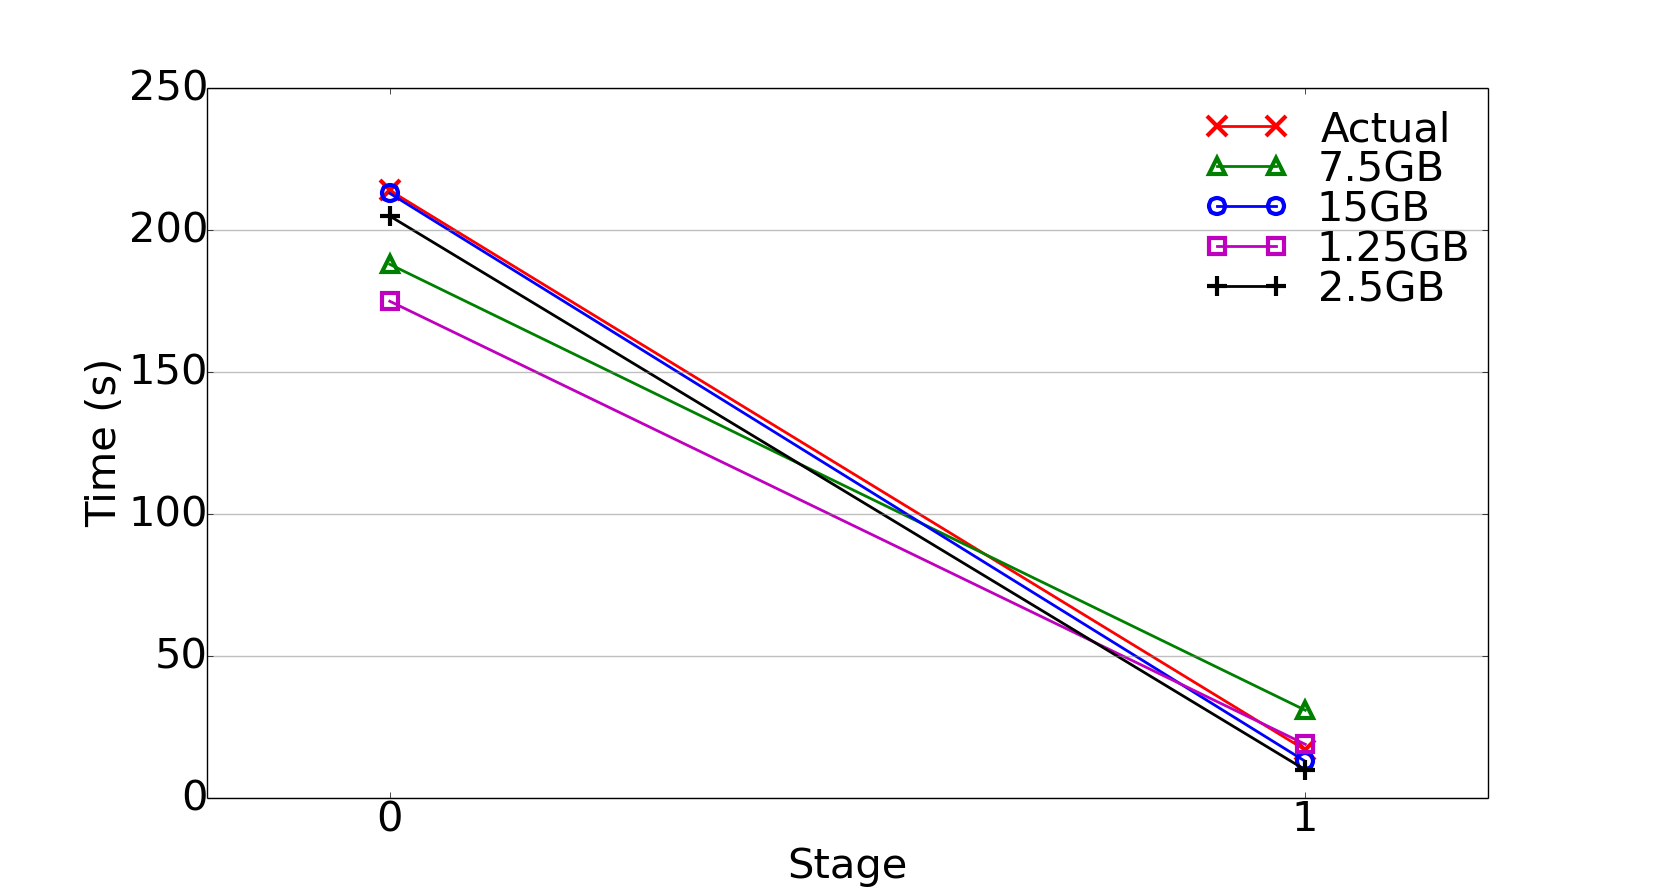
\includegraphics[width=3.5in]{figures/wc_time.png}
\caption{Time Prediction for WordCount}
\label{wc_time}
\end{figure}
\begin{figure}[!t]
\centering
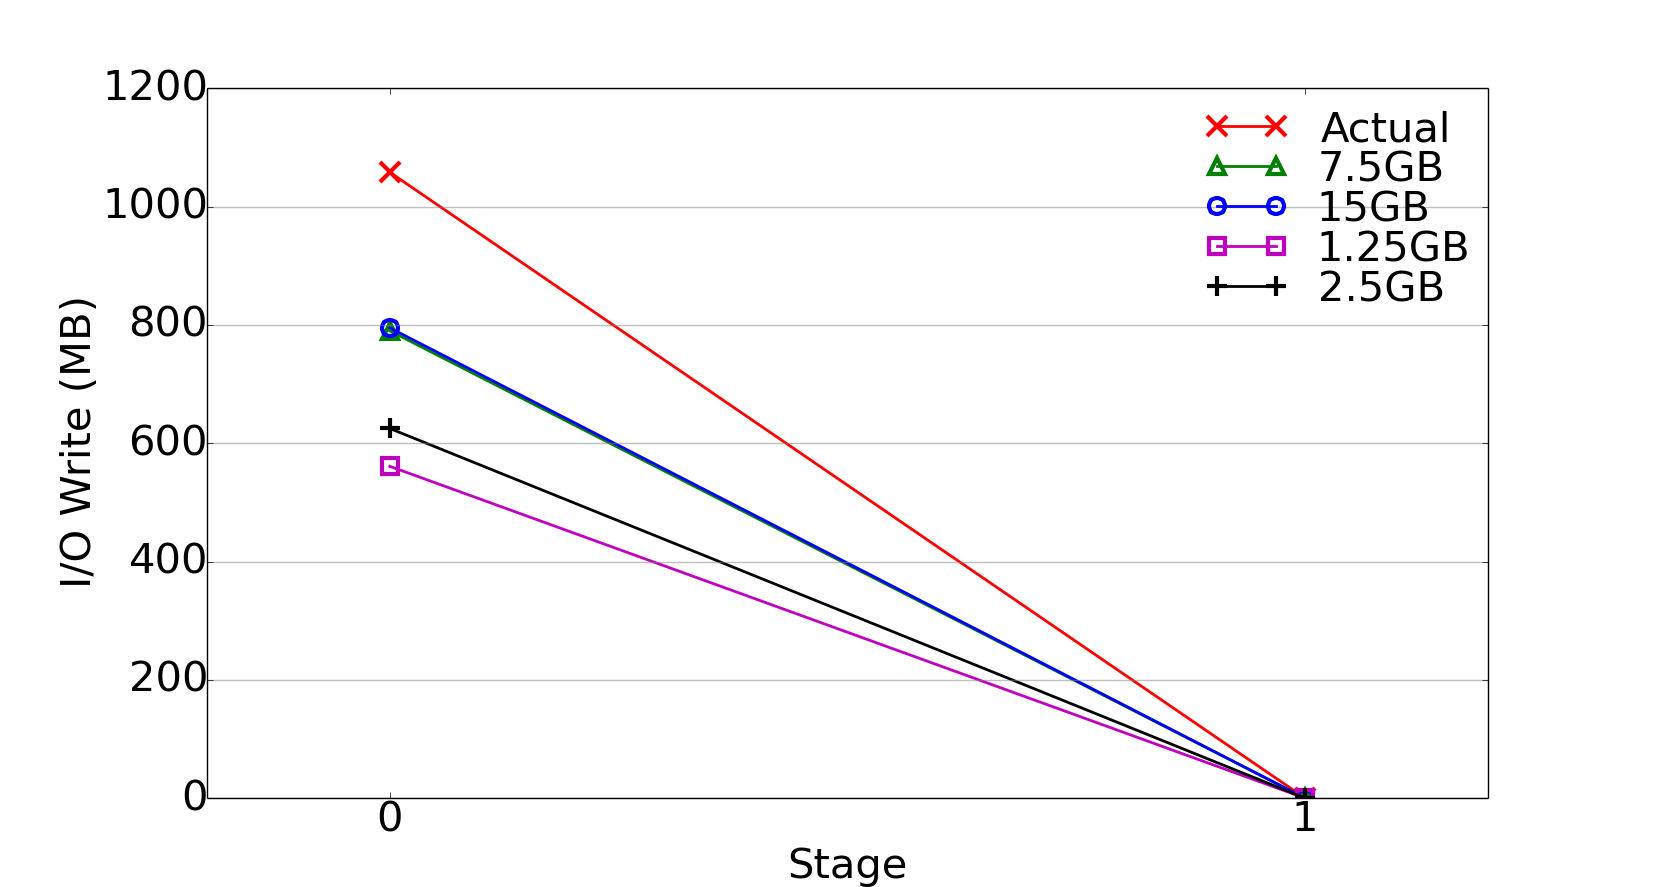
\includegraphics[width=3.5in]{figures/wc_io_w.png}
\caption{I/O Write Prediction for WordCount}
\label{wc_io_w}
\end{figure}
\begin{figure}[!t]
\centering
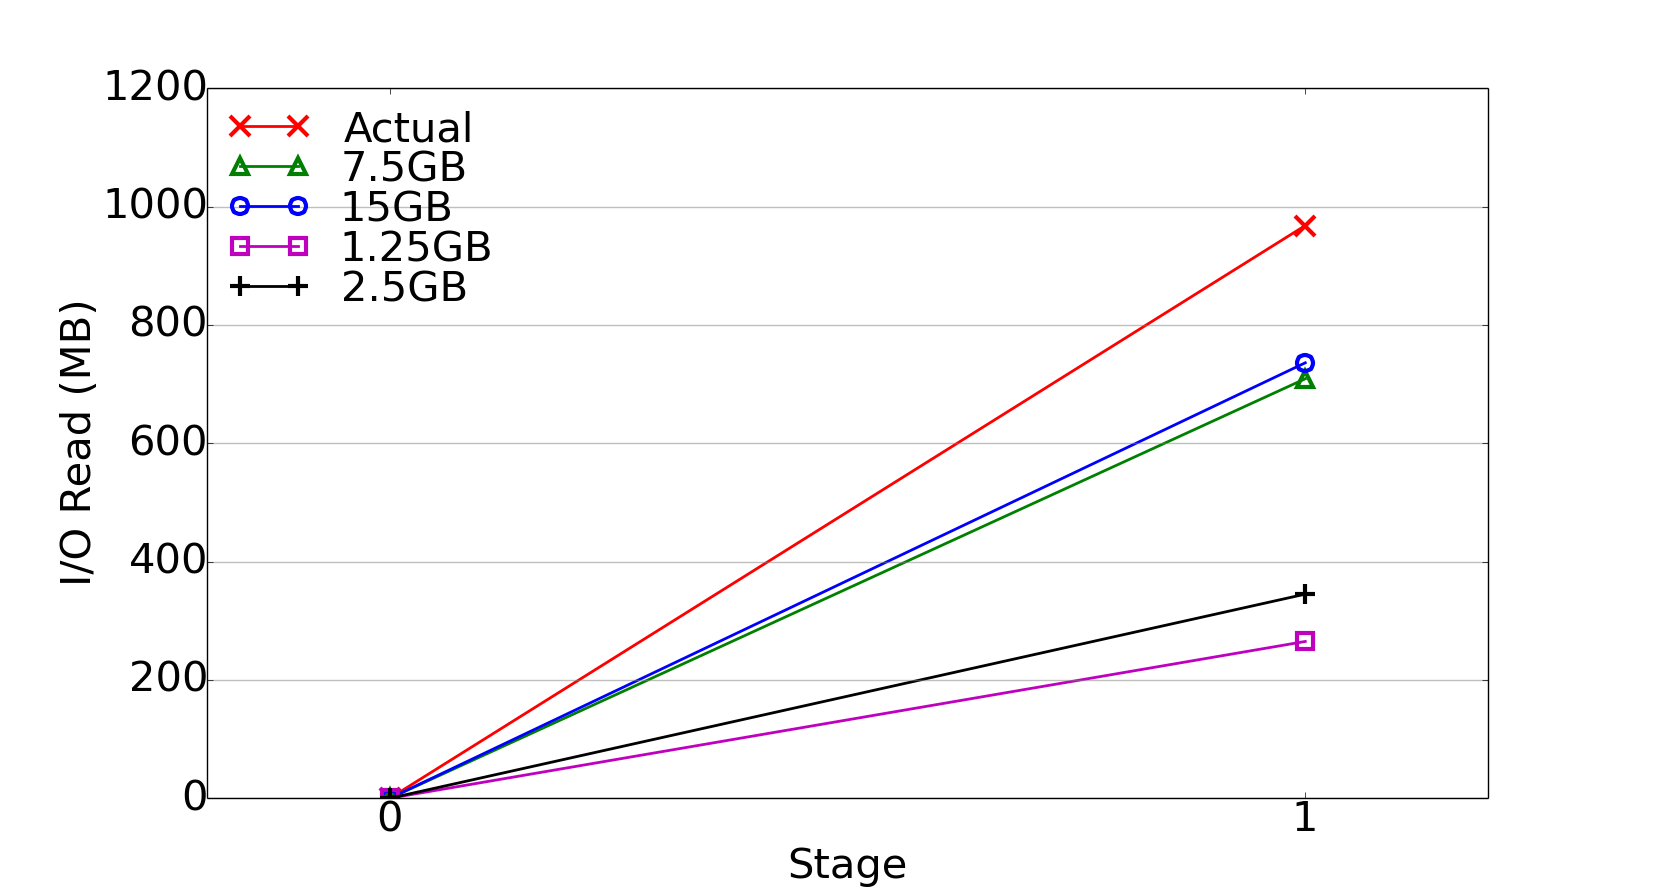
\includegraphics[width=3.5in]{figures/wc_io_r.png}
\caption{I/O Read Prediction for WordCount}
\label{wc_io_r}
\end{figure}


\subsection{Logistic Regression}

\noindent
Logistic Regression is an iterative algorithm with 10 stages, where there is no shuffle I/O cost. For Logistic Regression, the input data size is 50 GB. Figure~\ref{lr_accuracy} shows the prediction accuracy for execution time and memory usage for the whole job whereas Figure~\ref{lr_time} shows the actual and predicted execution time per stage. As logistic regression is a computing-intensive job, this minimizes the effect of I/O and leads to better prediction accuracy. For memory cost prediction, all four simulation setup achieved 100\% accuracy and correctly predicted the value of 11.5 GB needed to create the initial RDD (Figure~\ref{lr_accuracy}). 
\begin{figure}[!t]
\centering
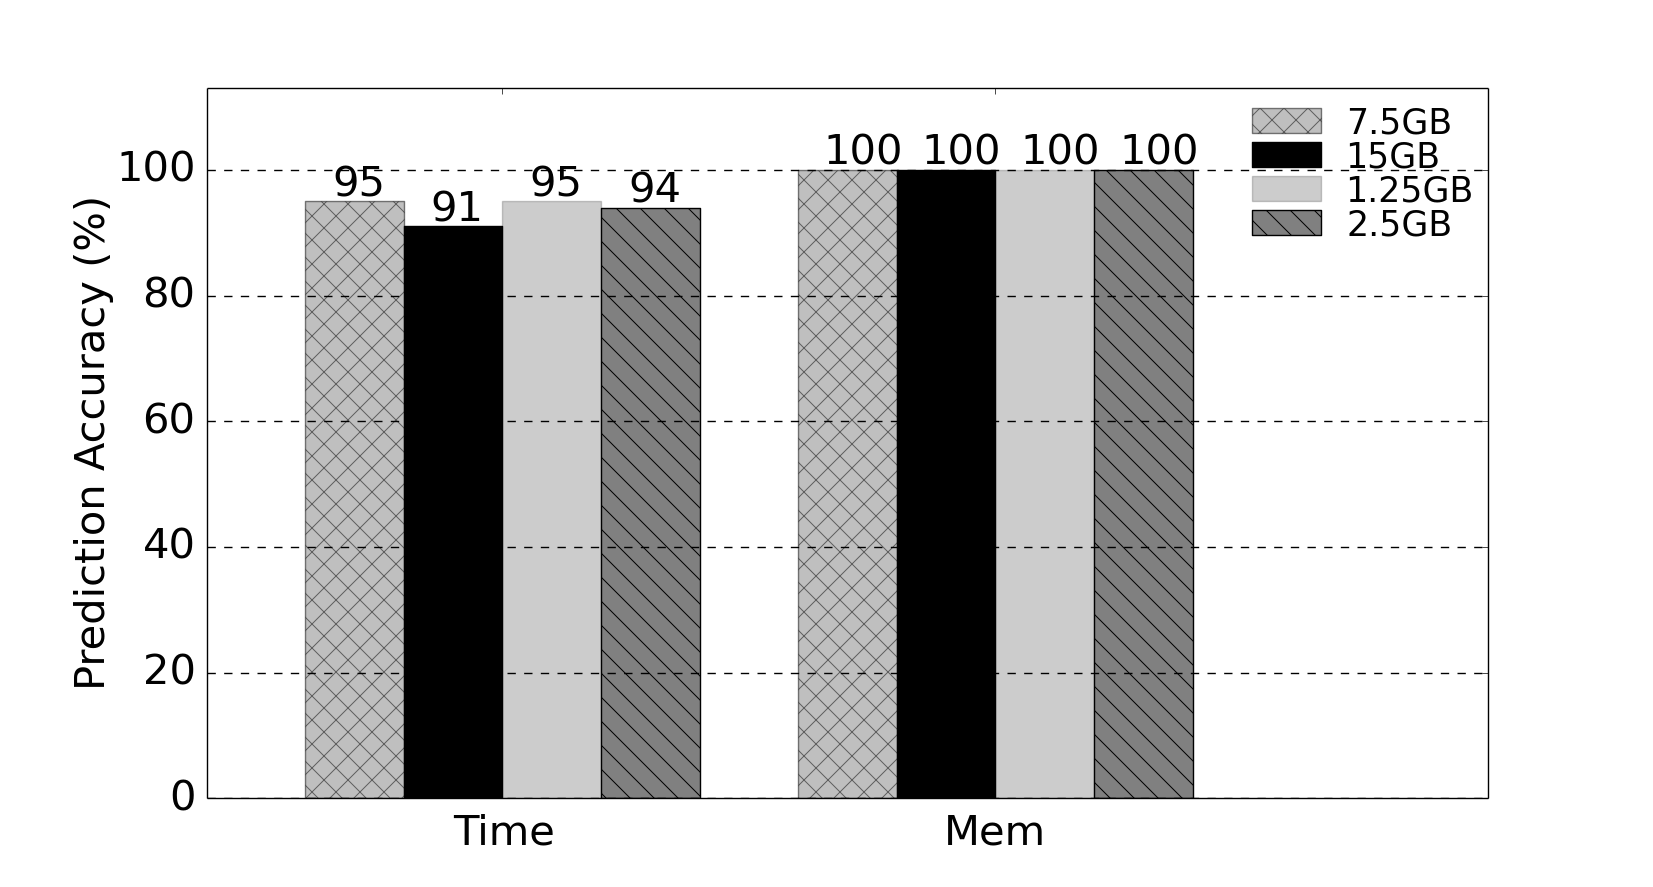
\includegraphics[width=3.5in]{figures/lr_accuracy.png}
\caption{Prediction Accuracy for Logistic Regression}
\label{lr_accuracy}
\end{figure}
\begin{figure}[!t]
\centering
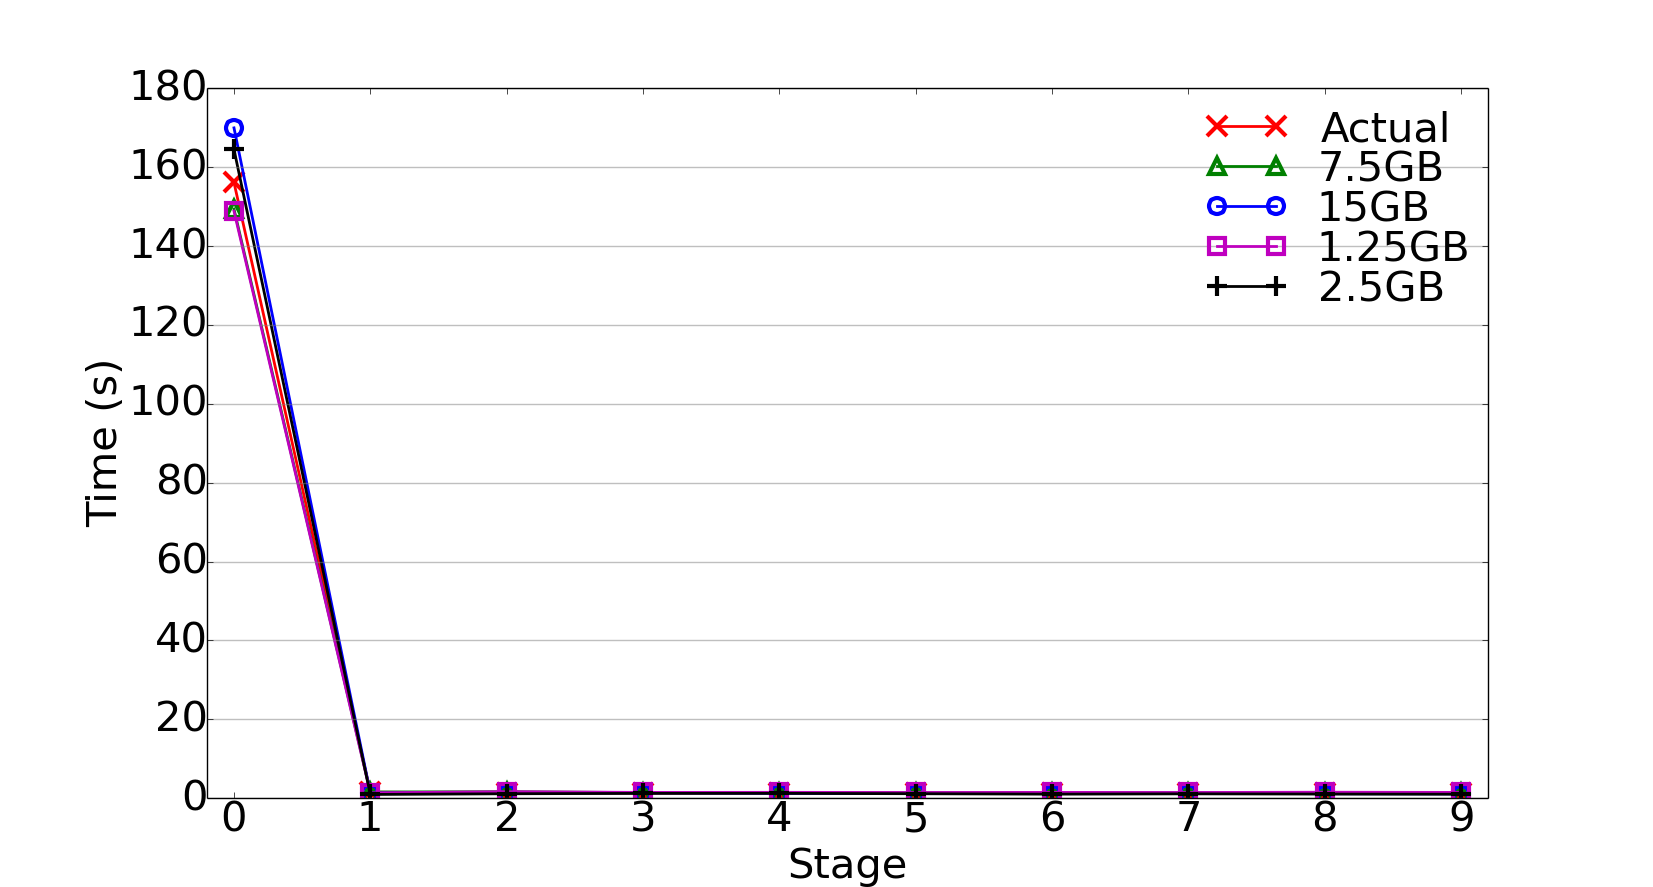
\includegraphics[width=3.5in]{figures/lr_time.png}
\caption{Time Prediction for Logistic Regression}
\label{lr_time}
\end{figure}


\subsection{K-Means}

\noindent
We use the same data set as input for K-Means clustering algorithm that was used for testing Logistic Regression algorithm. K-Means is an iterative algorithm with 22 stages. In the third stage of the job, the I/O cost involves shuffle write, and the I/O cost involves shuffle read in the fourth stage. Later stages follow the same pattern. Figure~\ref{km_accuracy} shows the prediction accuracy for execution time, memory usage, and I/O cost. Figure~\ref{km_time} shows the actual execution time along with predicted value for different stages. 
As the volume of data read and written was small (only few megabytes), the prediction error for I/O cost was high (Figure~\ref{km_io_w} and Figure~\ref{km_io_r}). However, as the time cost for I/O operations is small and has minimal effect on total execution time, the model still achieved high prediction accuracy for execution time. For memory cost prediction, the model had 100\% accuracy, correctly predicting the value of 11 GB (Figure~\ref{km_accuracy}).
\begin{figure}[!t]
\centering
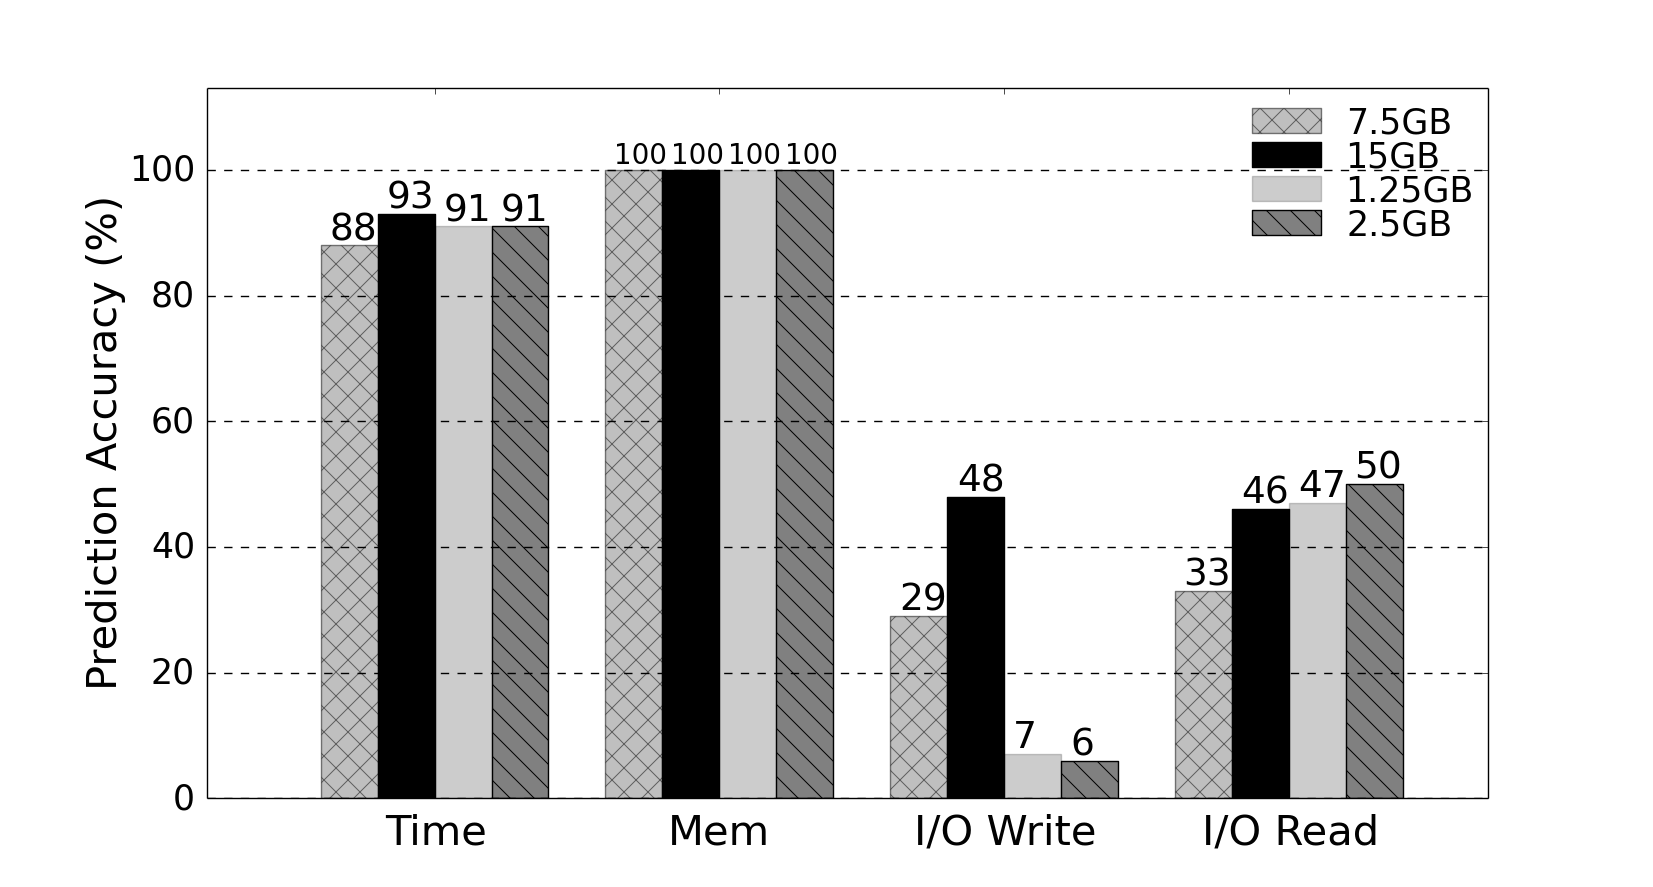
\includegraphics[width=3.5in]{figures/km_accuracy.png}
\caption{Prediction Accuracy for K-Means}
\label{km_accuracy}
\end{figure}
\begin{figure}[!t]
\centering
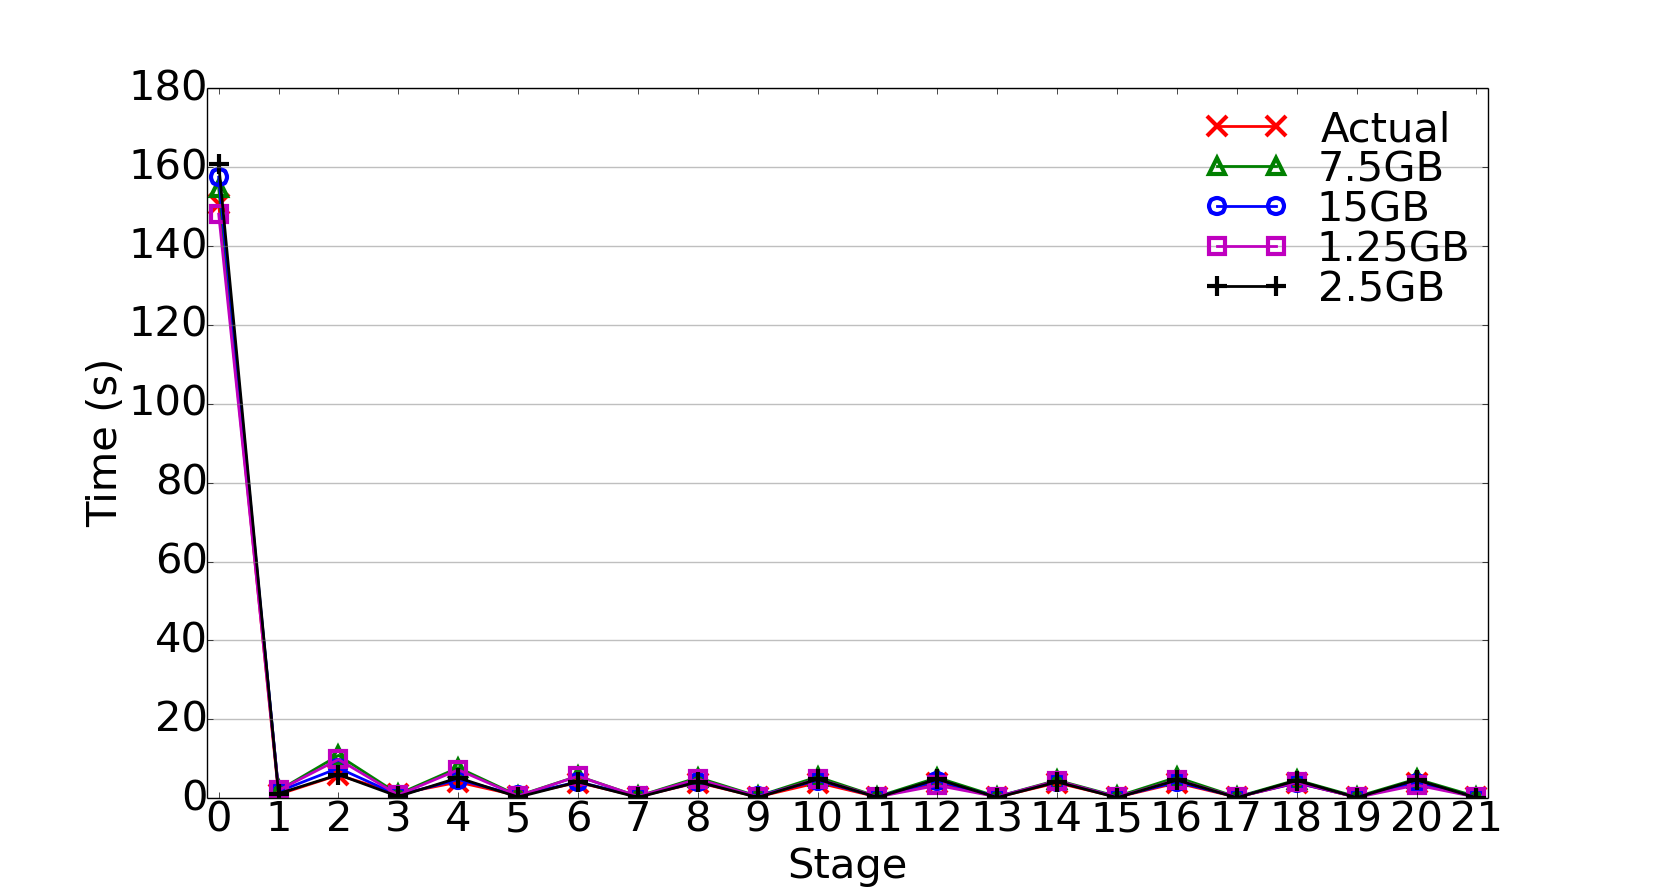
\includegraphics[width=3.5in]{figures/km_time.png}
\caption{Time Prediction for K-Means}
\label{km_time}
\end{figure}
\begin{figure}[!t]
\centering
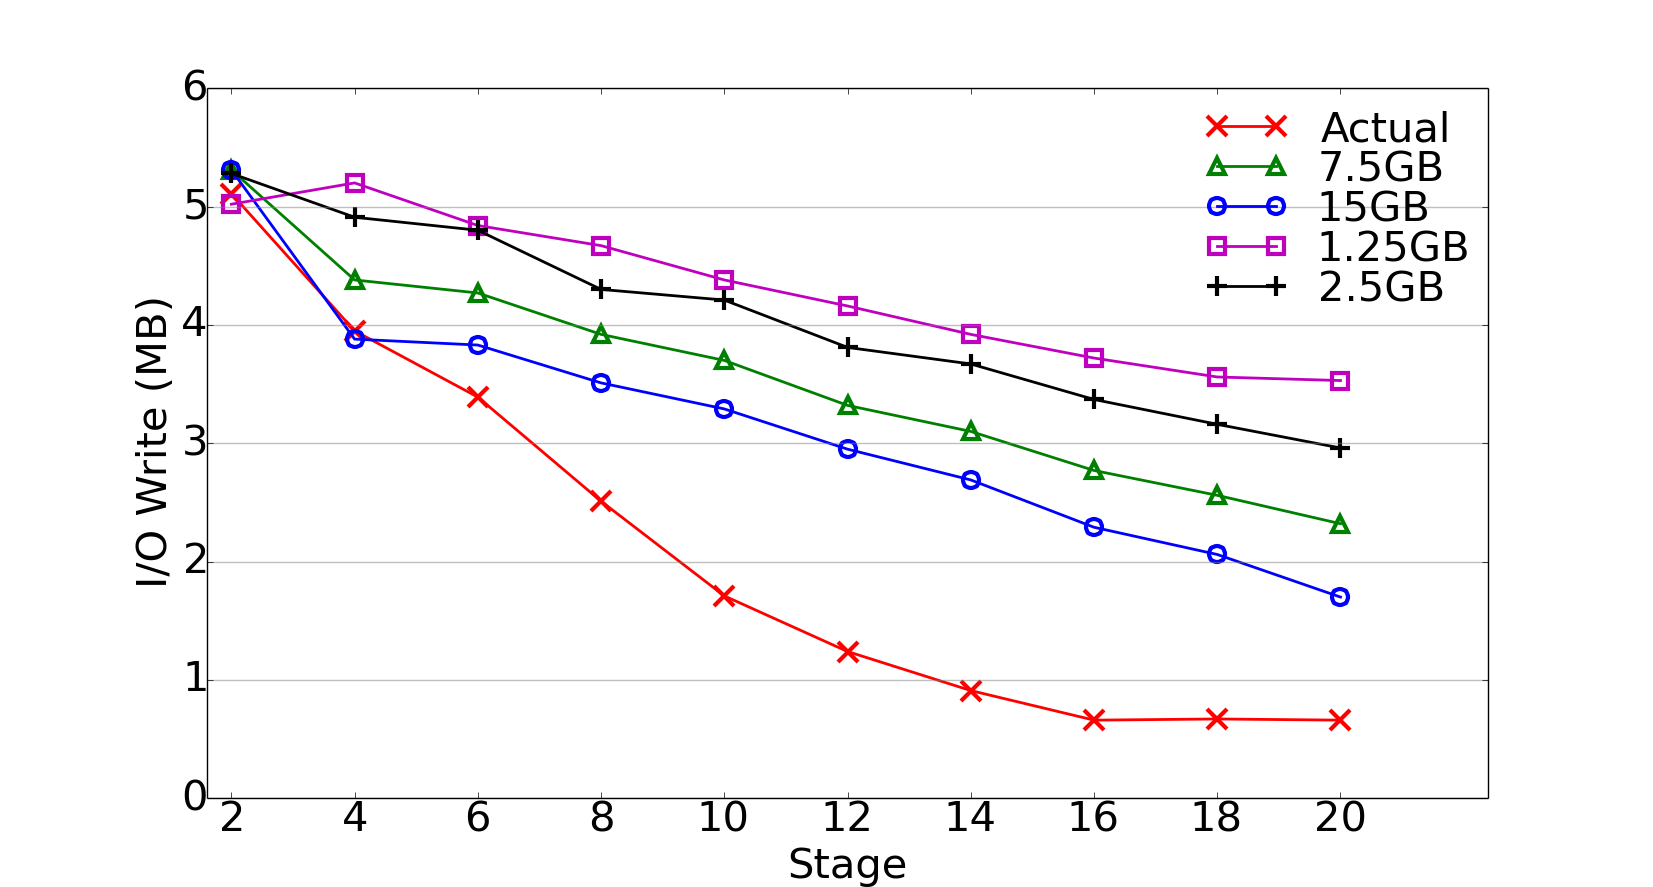
\includegraphics[width=3.5in]{figures/km_io_w.png}
\caption{I/O Write Prediction for K-Means}
\label{km_io_w}
\end{figure}
\begin{figure}[!t]
\centering
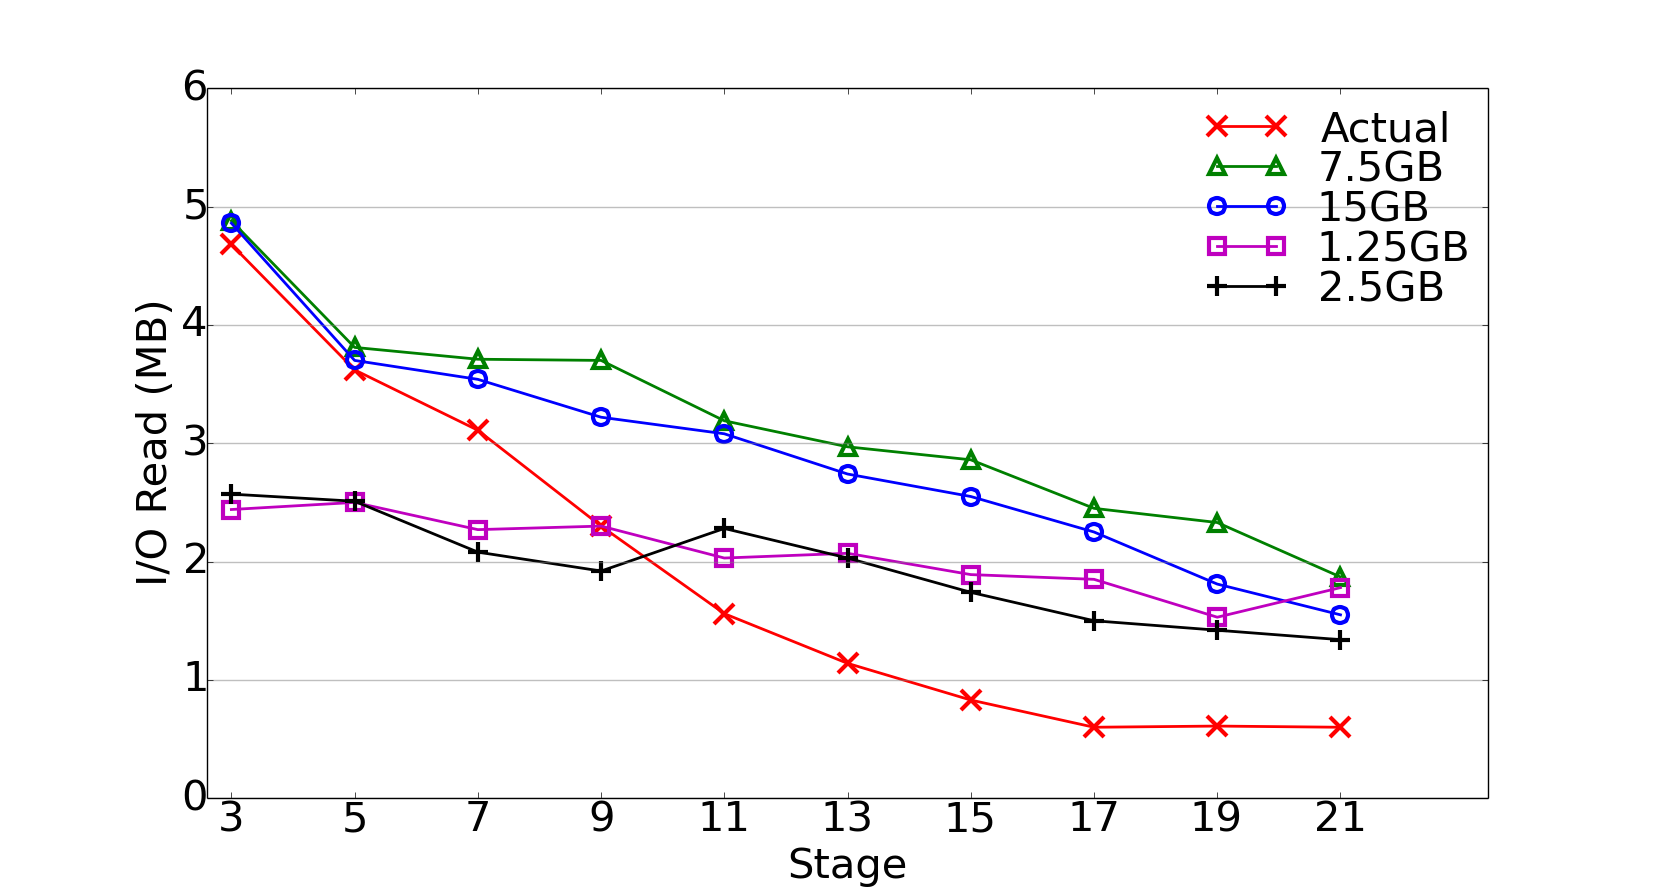
\includegraphics[width=3.5in]{figures/km_io_r.png}
\caption{I/O Read Prediction for K-Means}
\label{km_io_r}
\end{figure}
%Suppose $r_1$ is the change ratio of the average running time in second batch of tasks over the average time of the first batch and $r_2$ is another change ratio of the average running time in following batches of tasks over the average time of the first batch, which can be calculated in equation \ref{ratio}. $r_1$ is smaller than $r_2$ in this example. But we can only calculate $r_1$ because the size of sample data,which will bring the deviation in prediction. Actually, all the values of the predicted running time are smaller than the actual value in the experiment. In addition, the prediction accuracy could reach 99\% when using 100\% of the input data, which proves this explanation to some extent. 
%Comparing Fig.\ref{pr_io_r} and Fig.\ref{pr_io_w}, this accuracy gap is easily observed. The reason may be that shuffle read always incurs the network I/O cost for data fetching and shuffle write only generates local disk I/O for writing interim data to buckets. And smaller cluster can not capture the data transmission in the network of more worker nodes in large cluster.



\subsection{PageRank}

\noindent
PageRank is an iterative algorithm with 13 stages where there are I/O read and write costs for each stage. In our evaluation, we used 25 GB of input data. Figure~\ref{pr_accuracy} shows the prediction accuracy. For time prediction, the accuracy is above 80\% based on small scale simulation, but drops to around 70\% for the full cluster simulation (Figure~\ref{pr_accuracy} and Figure~\ref{pr_time}). This result may be due to the fluctuation in execution time across tasks within a stage. 
For I/O write cost prediction, the accuracy is above 90\% for large-scale simulation (Figure~\ref{pr_accuracy} and Figure~\ref{pr_io_w}). For memory cost prediction, the accuracy is close to 97\% for large-scale simulation (Figure~\ref{pr_accuracy}). However, the I/O read prediction is below 50\% based on small scale simulation (Figure~\ref{pr_accuracy} and Figure~\ref{pr_io_r}), which may be due to the inability to capture network activity in sufficient details in a small scale simulation.
\begin{figure}[!t]
\centering
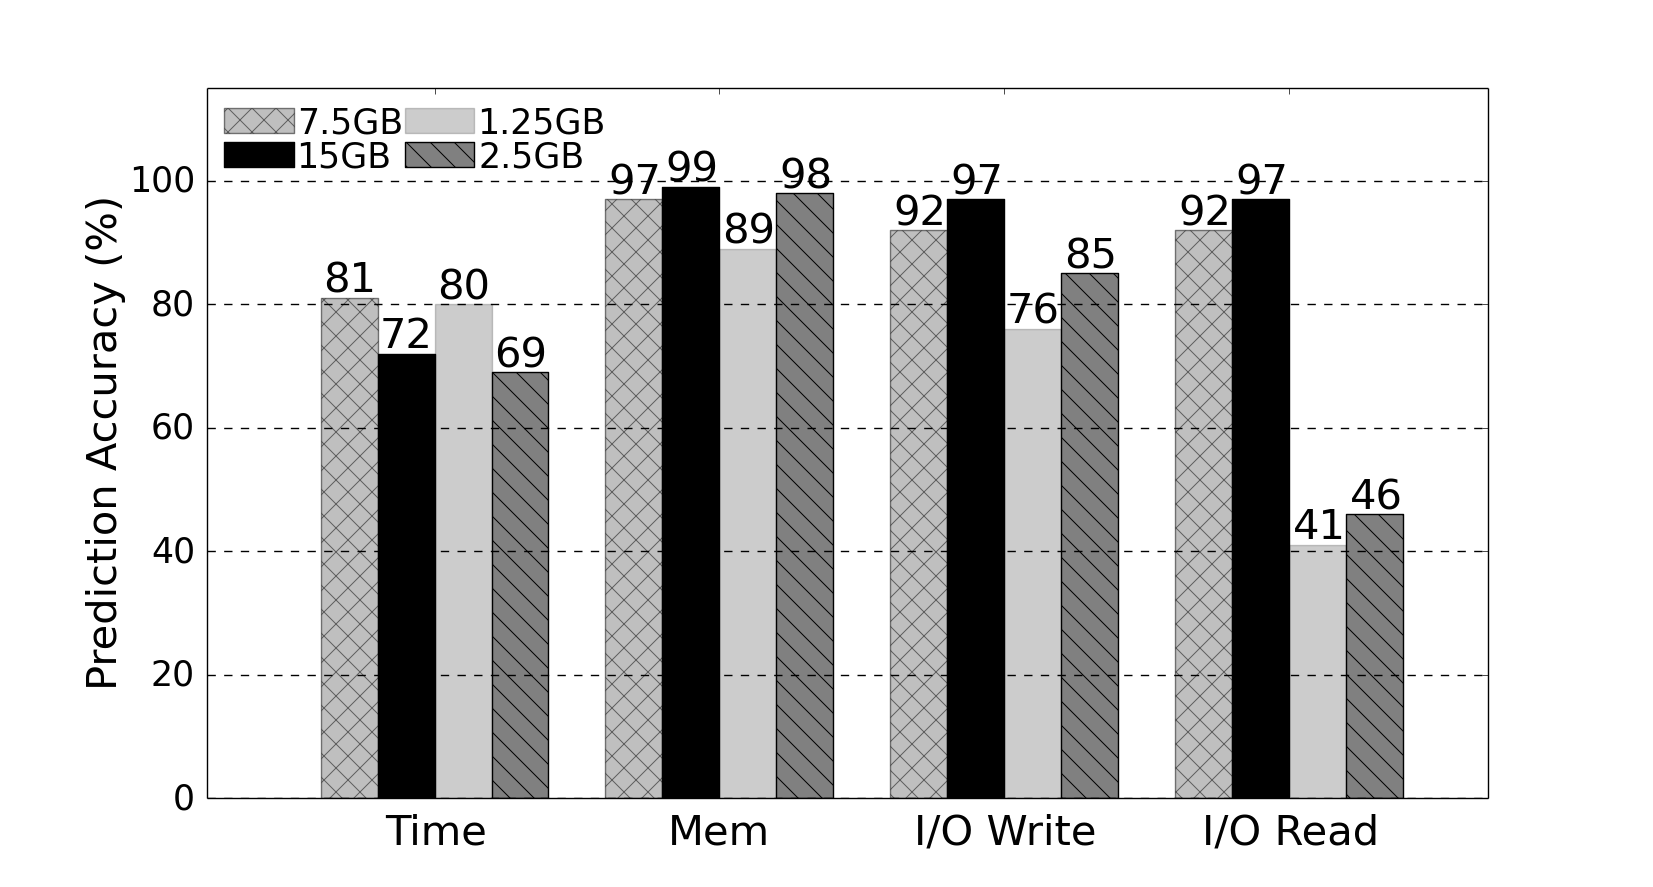
\includegraphics[width=3.5in]{figures/pr_accuracy.png}
\caption{Prediction Accuracy for PageRank}
\label{pr_accuracy}
\end{figure}
\begin{figure}[!t]
\centering
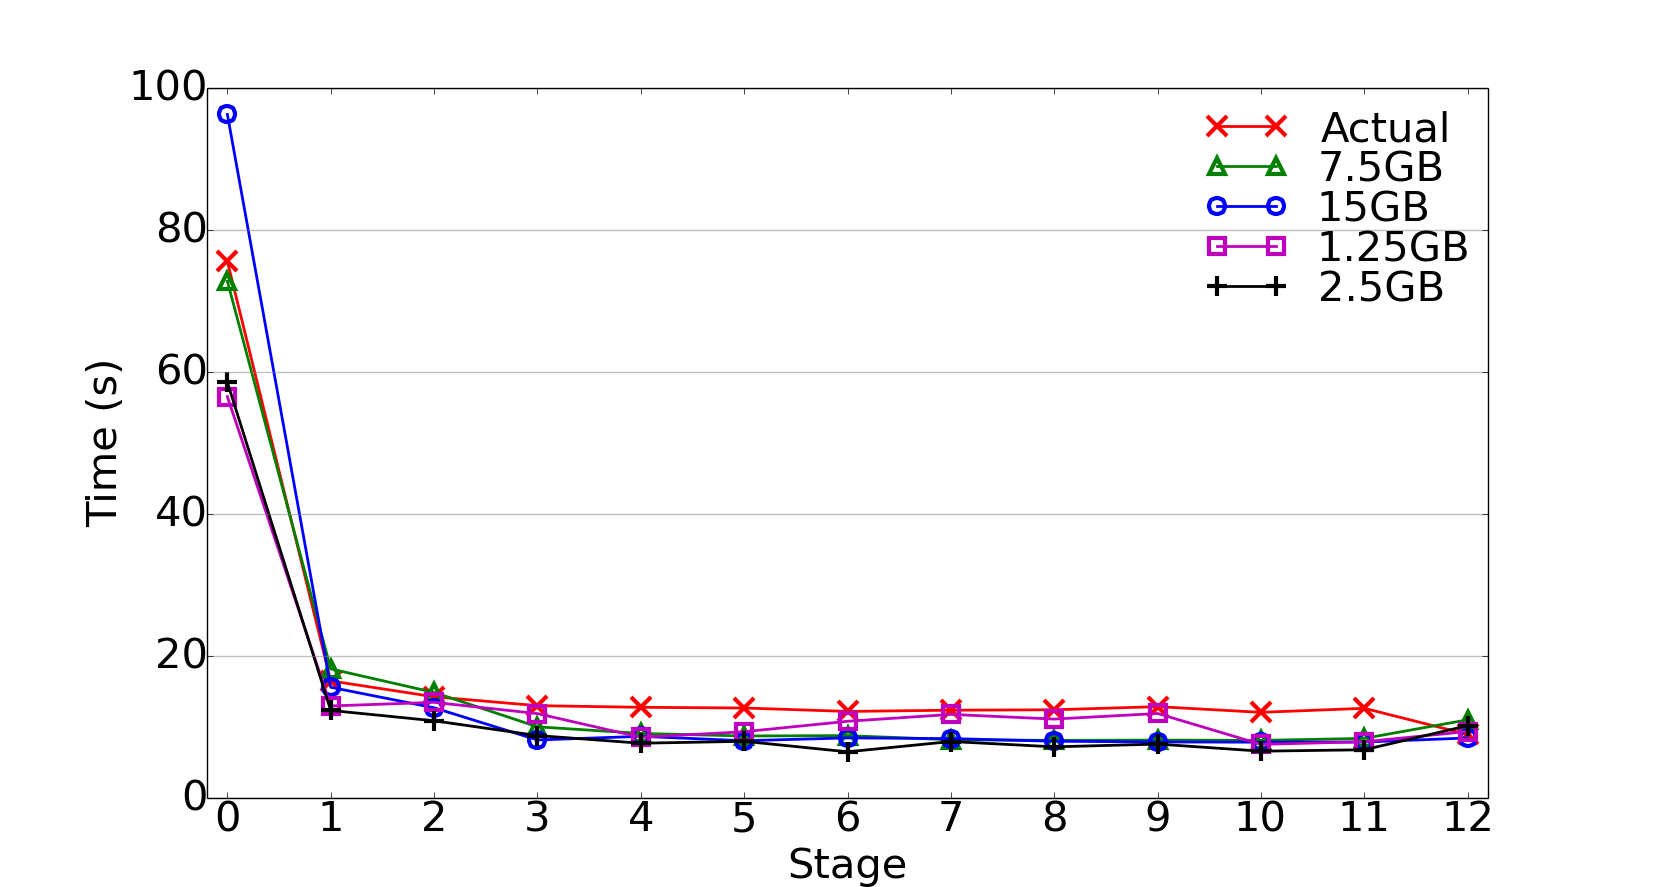
\includegraphics[width=3.5in]{figures/pr_time.png}
\caption{Time Prediction for PageRank}
\label{pr_time}
\end{figure}
\begin{figure}[!t]
\centering
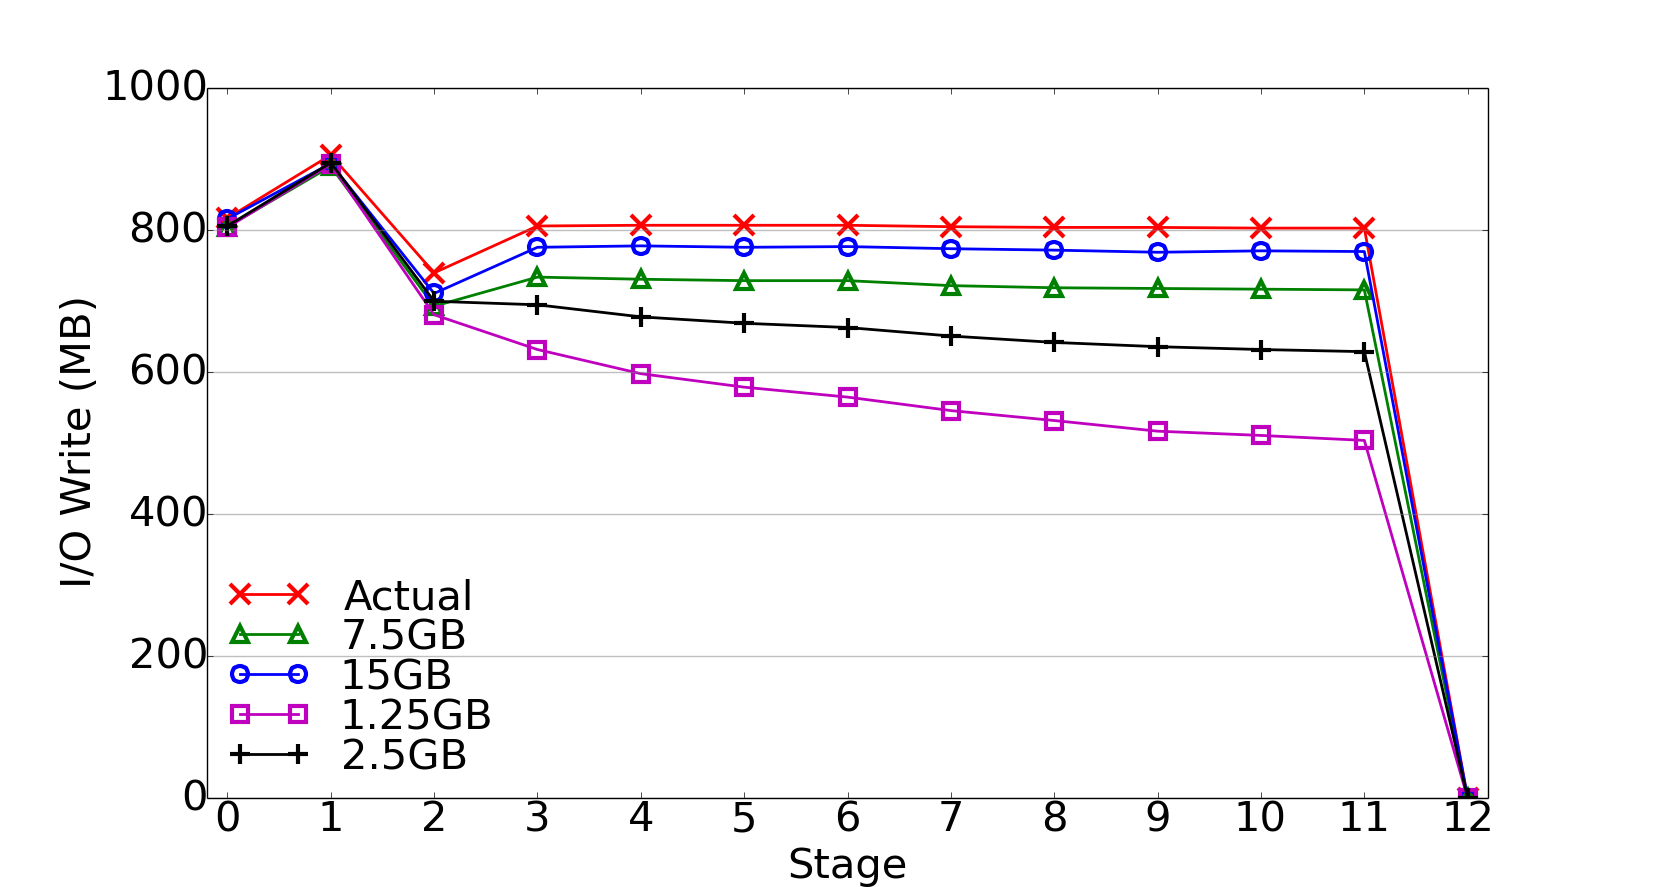
\includegraphics[width=3.5in]{figures/pr_io_w.png}
\caption{I/O Write Prediction for PageRank}
\label{pr_io_w}
\end{figure}
\begin{figure}[!t]
\centering
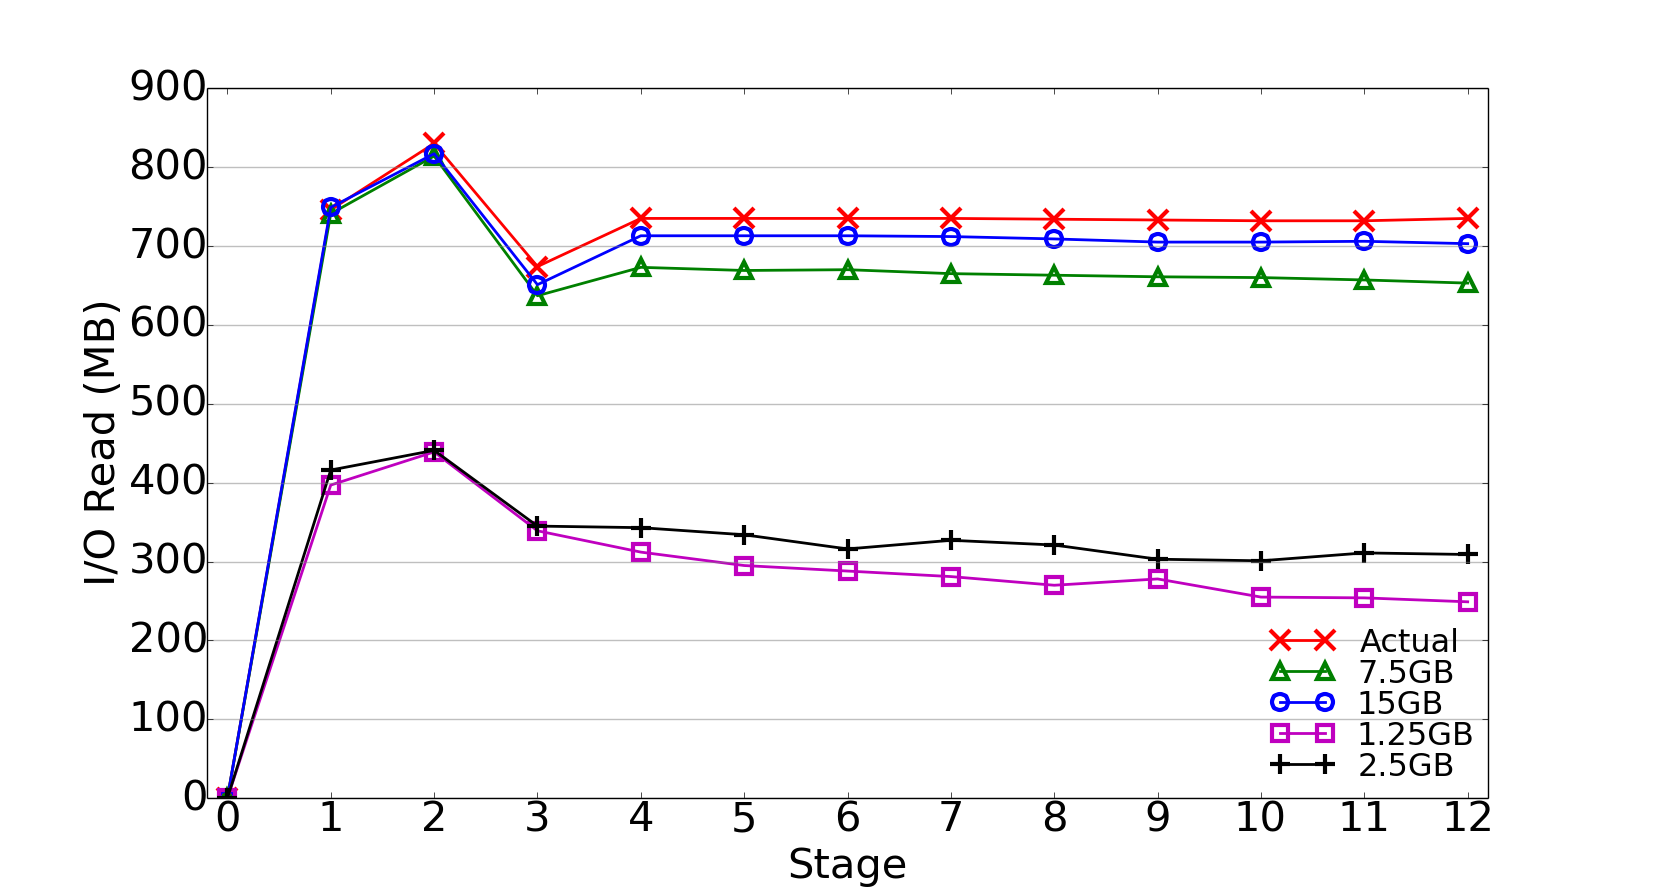
\includegraphics[width=3.5in]{figures/pr_io_r.png}
\caption{I/O Read Prediction for PageRank}
\label{pr_io_r}
\end{figure}
%\begin{figure}[!t]
%\centering
%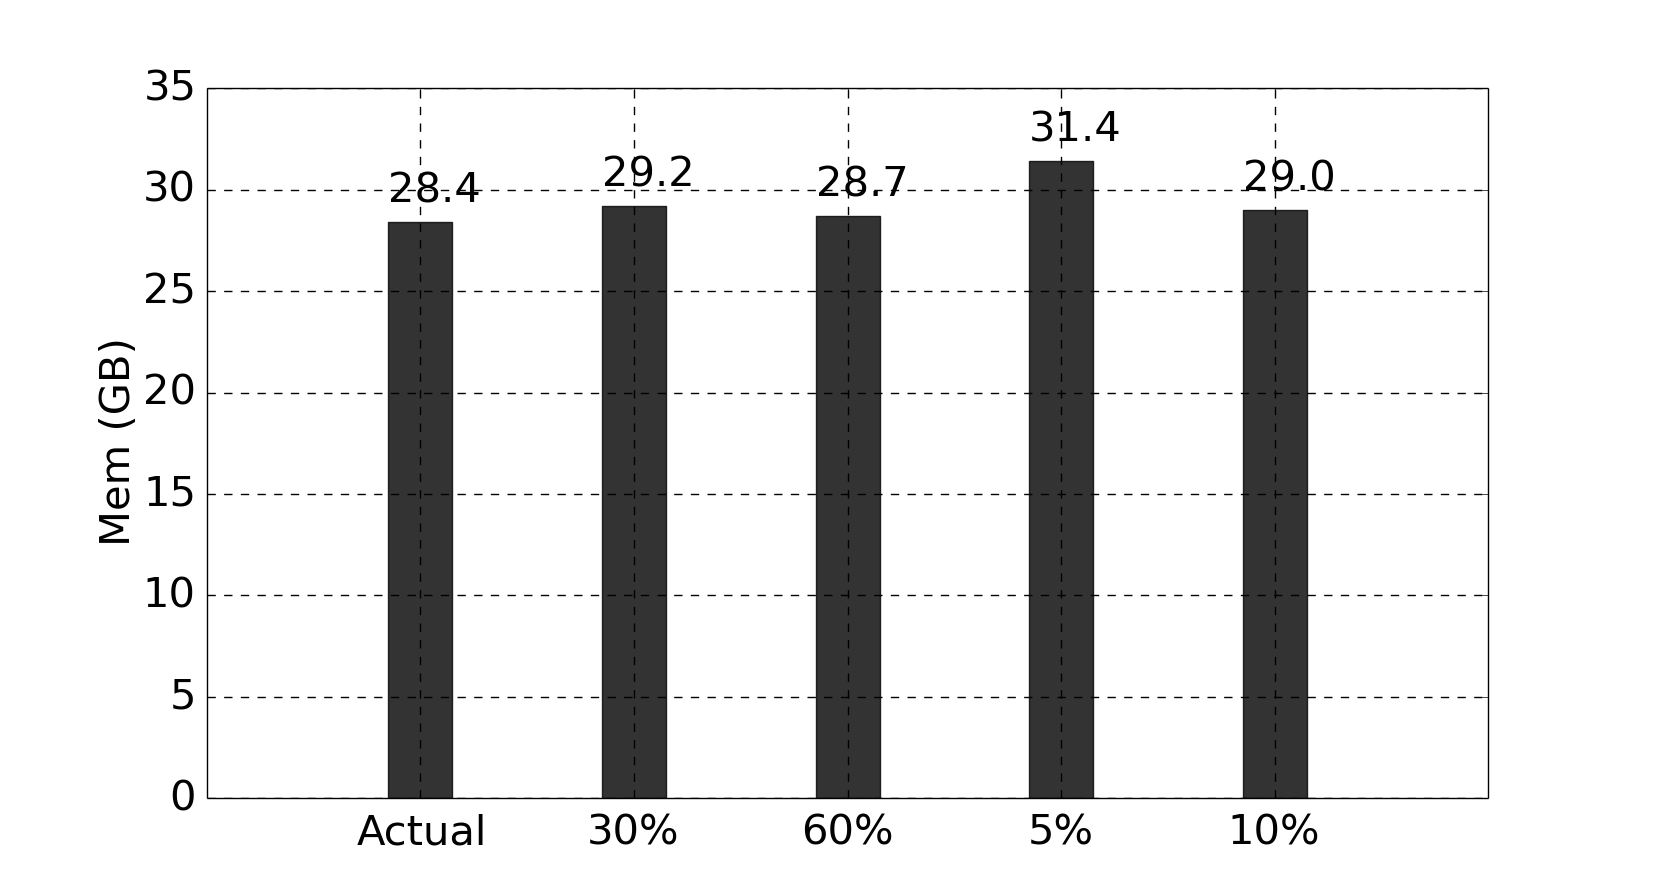
\includegraphics[width=3.0in]{figures/pr_mem.png}
%\caption{Memory Cost Prediction for PageRank}
%\label{pr_mem}
%\end{figure}

